\renewcommand{\thesection}{\Alph{section}}
\section{Product perspective}\label{sec:product_perspective}
\subsection{Scenarios}\label{subsec:scenarios}
\subsubsection{Scenario 1: Mr.Spongebob registers on the platform}\label{subsubsec:scenario_1}
Mr.Spongebob, a final-year student at the University of Bikini Bottom, is looking for an internship to practice the knowledge he's gained. 
To do so, he asks advice from Professor Puff, who suggests using the Students\&Companies platform to search for internship opportunities.
Following her advice, Mr.Spongebob registers as a student on the platform, selecting the University of Bikini Bottom from the list of 
universities and verifying his student status with his educational email and password. Then, he fills in all the required personal information,
including his name, date of birth, and other details. He also inserts keywords to describe his skills and the job fields he might be interested 
in. Finally, after uploading his CV, which contains all the necessary information and details, Mr.Spongebob completes his registration and 
can begin searching for internships. Meanwhile, Professor Puff, who oversees internship activities using the official account of the University of 
Bikini Bottom, is notified of Mr.Spongebob's registration.

\subsubsection{Scenario 2: Mr.Krabs publishes an internship offer}\label{subsubsec:scenario_2}
Due to the rapid evolution of Technology, Mr.Krabs decides to collaborate with his competitor Mr.Plankton, on a new project. They 
plan to develop a ``Hamburger super secret formula detector'' that can detect what the customer likes by looking at his facial expressions, in 
order to to create the perfect personalized hamburger! To achieve this, they need to hire students specializing in Computer Vision, Deep Learning and
AI to study the visual data. So Mr.Krabs logs into the Students\&Companies platform using the official company account
and navigates to the ``Publish Internship'' section to create a new announcement. He fills in all the required information: 
the title, location, role, application deadline, number of positions, duration, employment type, description, and required skills.
After that, Mr.Krabs published the internship offer, which can be seen in the ``Available Internships'' section. Immediately after 
the publication, he receives a notification of recommended student profiles that may match the offer requirements.
\begin{quote}
    \begin{center}
       \textbf{\textquotedbl Computer Vision and AI Intern\textquotedbl}
    \end{center}
    
    \textit{Location:} Krusty Krab Technology Lab, Bikini Bottom \\
    \textit{Role:} Intern \\
    \textit{Application Deadline:} 25th December 2024 \\
    \textit{Number of Positions:} 2 \\
    \textit{Duration:} 6 months \\
    \textit{Employment Type:} Full-time \\
    \textit{Description:} We are looking for students who can contribute to the development of the Hamburger super secret formula detector by developing 
    algorithms that collect and analyze visual data. A love for hamburgers is essential!\\
    \textit{Required Skills:} Computer Vision, AI, Python, Deep Learning
\end{quote}

\subsubsection{Scenario 3: Mr.Patrick searches internship}\label{subsubsec:scenario_3}
Mr.Patrick is very worried because he is in the last semester of his master's degree, so he has to find an internship or he won't be able to graduate in Food Engineering.
He remembers he has an account on the Students\&Companies platform, which he used to find an internship at the beginning of his studies, so he decides 
to take another look at the platform. He logs in and updates his profile and CV, adding the new skills he has acquired during his master’s degree.
He navigates to the search bar and types ``Hamburger'' to look for internships related to hamburger studies. When he doesn’t find anything that 
interests him, he scrolls through the recommended internships list. Finally, he finds Mr.Krabs' posting and becomes very interested in the 
project, so he applies for the internship and waits for the company's response. After applying, he can check the status of his application in 
the ``Your Applications'' section.

\subsubsection{Scenario 4: Krusty Krab Technology Lab Interview}\label{subsubsec:scenario_4}
After the application deadline, Mr.Krabs and Mr.Plankton review all the applications received for the intern position. They select the
candidates by reviewing their profiles and CVs, and then send them an invitation for an interview. For the first round of interviews, Mr.Plankton
decides to formulate a set of short questions to know more about the candidates' skills and experiences. The candidate will be able to respond to 
these questions through a form inside the platform. In said form Mr.Plankton also includes the date, time and location of the interview and the 
necessary information to better prepare the candidates. After sending the invitations, the candidates selected for the interview receive a notification 
from the platform, who is not selected will receive a notification of rejection. At the end of the interview, Mr.Plankton evaluates the candidates 
and discusses with Mr.Krabs to decide who to hire. Finally, they send an offer to the best candidates and wait for their acceptance to start the internship.

\subsubsection{Scenario 5: Ms.Sandy starts her internship}\label{subsubsec:scenario_5}
Ms.Sandy is very passionate about space and is thrilled to have been selected for an internship at the Underwater Space Agency. She receives 
and accepts an offer from the company. At the same time, the Bikini Bottom University of Aerospace's professor Manta received the notification
about the new activity started by Sandy. However, she is a bit anxious, so she logs into the platform and navigates to the ``Internship'' 
section to find her assigned mentor's profile. She starts a chat with him to ask some questions about how she should prepare in the coming days
and for any advice he can give her to have a good start in the internship.

\subsubsection{Scenario 6: Mr.Squidward leaves his feedback}\label{subsubsec:scenario_6}
At the end of his internship at the ``Krusty Krab Technology Lab'' as a data science intern, Mr.Squidward is surprised by the experience 
he has gained, even though he has several complaints about the heavy workload. He decides to leave a warm message for Mr.Krabs and Mr.Plankton 
to thank them for the opportunity. After that, he navigates to the ``Internship'' section to add a review of his internship experience and rate 
the company. It is also the section where he can check the suggestions left by his mentors regarding his internship, which is only visible to the 
company and the university.

\subsubsection{Scenario 7: Track the internship activities}\label{subsubsec:scenario_7}
As the internship period progresses, Professor Puff is responsible for overseeing the students' activities at the University of Bikini Bottom. 
She is curious to know how the students are doing in their internships, particularly Mr.SpongeBob, who is using the platform for the first time. 
She logs into the platform with the university credentials and looks at the list of students, searching for SpongeBob's name. She finds, 
in his active internship section, that he has been selected for an internship at the ``Krusty Krab Technology Lab''. By reading the feedback 
left by the company throughout the different stages of the internship, she is very glad to see that SpongeBob is doing well in the field he is 
passionate about!


\subsection{Domain-level diagram}\label{subsec:domain_level_diagram}
%TODO add domain-level diagram

\subsection{Statecharts}\label{subsec:statecharts}

\subsubsection{1. Internship recommendation}\label{subsubsec:internship_application}
\begin{figure}[H]
    \centering
    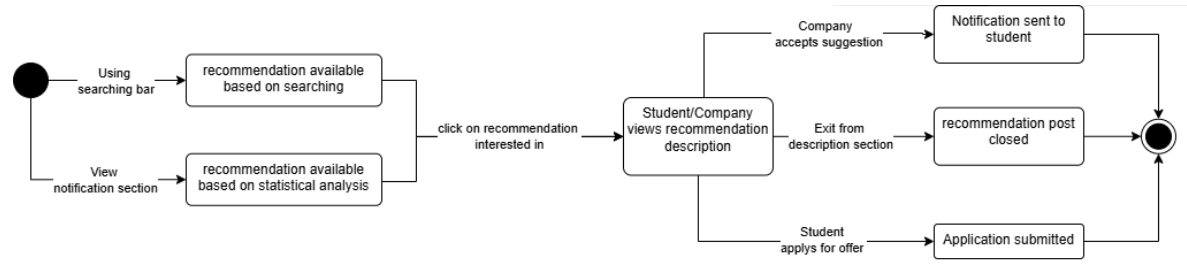
\includegraphics[width=1\textwidth]{Images/Internship_recommendation.png}
    \caption{Statechart diagram for internship recommendation}\label{fig:statechart_internship_recommendation}
\end{figure}
%TODO add description

\subsubsection{2. Selection process for internship}\label{subsubsec:internship_feedback}
\begin{figure}[H]
    \centering
    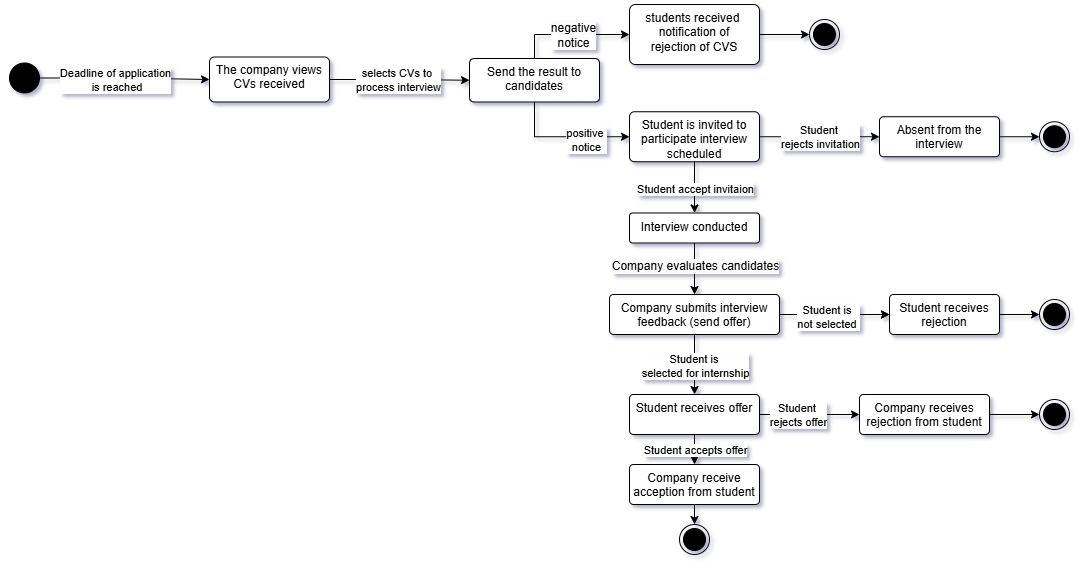
\includegraphics[width=1\textwidth]{Images/Selection_process.png}
    \caption{Statechart diagram for selection process for internship}\label{fig:statechart_selection_process_for_internship}
\end{figure}
%TODO add description

\subsubsection{3. Internship status}\label{subsubsec:monitoring_student_activities}
\begin{figure}[H]
    \centering
    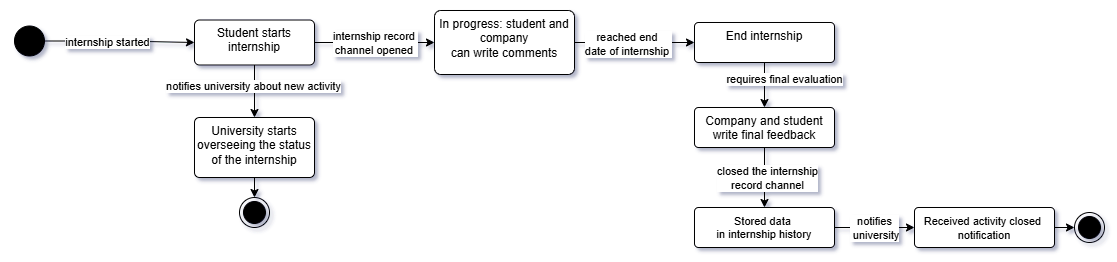
\includegraphics[width=1\textwidth]{Images/Internship_status.png}
    \caption{Statechart diagram for internship status}\label{fig:statechart_internship_status}
\end{figure}
%TODO add description

\section{Product functions}\label{subsec:product_functions}
\begin{itemize}
    \item \textbf{Sign up and login} 
    \item \textbf{Data management system}
    \item \textbf{Search system} 
    \item \textbf{Recommendation system} 
    \item \textbf{Internship application} 
    \item \textbf{Internship Posting}
    \item \textbf{Selection Assistance} 
    \item \textbf{Internship Status Tracking} 
    \item \textbf{Internship Feedback}
    \item \textbf{Monitoring student activities} 
    \item \textbf{Chat system} 
    \item \textbf{Notification system} 
    \item \textbf{Application Acceptance and Rejection} 
\end{itemize}

\section{User characteristics}\label{subsec:user_characteristics}


\section{Domain Assumptions}\label{subsec:domain_assumptions}